\documentclass[11pt]{article}
\usepackage[margin=1in]{geometry}
\usepackage[utf8]{inputenc}
\usepackage[T1]{fontenc}
\usepackage{hyperref}
\usepackage{url}
\usepackage{booktabs}
\usepackage{amsfonts}
\usepackage{microtype}
\usepackage{graphicx}
\usepackage{float}
\usepackage{natbib}
\usepackage{authblk}
\usepackage{tikz}
\usetikzlibrary{positioning, arrows.meta, fit, backgrounds}

\title{Adapting VACE for Real-Time Autoregressive Video Generation}

\author[1]{Ryan Fosdick\thanks{ryan@livepeer.org}}
\affil[1]{Daydream Live}

\date{}

\begin{document}

\maketitle

\begin{abstract}
We describe an adaptation of VACE (Video All-in-one Creation and Editing) for real-time autoregressive video generation. VACE provides unified video control---reference guidance, structural conditioning, inpainting, and temporal extension---but assumes bidirectional attention over full sequences, making it incompatible with streaming pipelines that require fixed chunk sizes and causal attention. The key modification moves reference frames from the diffusion latent space into a parallel conditioning pathway, preserving the fixed chunk sizes and KV caching that autoregressive models require. This adaptation reuses existing pretrained VACE weights without additional training. We observe 17--22 FPS throughput at $368 \times 640$ resolution on an NVIDIA RTX 5090 depending on mode, with structural control and inpainting at ${\sim}$17 FPS and temporal extension at ${\sim}$22 FPS. Reference-to-video fidelity is reduced compared to batch VACE due to causal attention constraints. A reference implementation is available at \url{https://github.com/daydreamlive/scope}.
\end{abstract}

\section{Introduction}

Real-time video generation models such as LongLive~\citep{yang2026longlive}, Krea Realtime Video~\citep{millon2025krea}, and StreamDiffusion V2~\citep{feng2025streamdiffusionv2} generate video autoregressively in chunks using causal attention. Each chunk attends only to itself and past frames, enabling KV caching and bounded memory usage. However, these models lack the control capabilities available to batch video generation models: reference guidance, structural conditioning, and selective editing. Building these capabilities from scratch would require extensive retraining.

VACE~\citep{jiang2025vace} provides unified video control for batch-oriented diffusion models, supporting reference-to-video generation, video-to-video structural control, masked editing (inpainting/outpainting), temporal extension, and arbitrary compositions of these capabilities. However, VACE assumes bidirectional attention and processes full video sequences at once, making it incompatible with streaming generation.

This paper presents an adaptation that enables VACE's control capabilities in streaming autoregressive pipelines. The technique is general to any chunked autoregressive diffusion model with causal attention and is not tied to a specific application or product. Our contributions are:

\begin{itemize}
    \item An architectural modification that moves reference frames from the diffusion latent space into a parallel conditioning pathway, resolving the incompatibility between VACE's reference handling and fixed-size chunk processing.
    \item Demonstration that pretrained VACE Context Block weights transfer directly to the adapted architecture without fine-tuning, due to the preservation of zero-initialized hint injection structure.
    \item Empirical validation that structural control (depth, scribble, optical flow, layout), masked generation (inpainting, outpainting), and temporal extension all function at real-time rates (17--22 FPS) on consumer hardware in streaming contexts.
    \item Empirical validation across Wan2.1 1.3B and 14B model scales using the same adaptation code without per-model modifications.
\end{itemize}

This work does not retrain VACE or introduce new control modules. It provides an architectural adaptation that enables pretrained VACE Context Blocks to function in causal chunked pipelines without modifying base model weights.

\section{Background}

\subsection{Autoregressive Video Generation}

Autoregressive video diffusion models~\citep{yang2026longlive, ji2025memflow, lu2025rewardforcing} generate video in fixed-size chunks using causal attention patterns. Each chunk of latent frames is denoised conditioned on cached key-value pairs from previously generated chunks. This design enables streaming generation with bounded memory, but constrains the model to causal (past-only) attention.

\subsection{VACE: Unified Video Control}

VACE~\citep{jiang2025vace} unifies video control through three optional conditioning inputs combined with a text prompt:

\begin{itemize}
    \item \textbf{Source video} (\texttt{src\_video}): Conditioning signal such as depth maps, pose skeletons, or video to edit.
    \item \textbf{Source mask} (\texttt{src\_mask}): Defines reactive (white, to be generated) vs.\ inactive (black, to be preserved) regions.
    \item \textbf{Reference images} (\texttt{src\_ref\_images}): Style or subject guidance images.
\end{itemize}

VACE processes these inputs through a parallel set of transformer blocks (Context Blocks) that produce ``hints''---additive signals injected into the main Diffusion Transformer (DiT)~\citep{peebles2023dit} pathway via zero-initialized linear projections. The base DiT is frozen; only the Context Blocks are trained (Context Adapter Tuning).

The publicly released VACE weights target the Wan video generation model~\citep{wang2025wan}, which provides 1.3B and 14B parameter variants with a 3D VAE~\citep{kingma2013vae} for temporal compression.

\section{The Architectural Problem}

\subsection{Reference Handling in Original VACE}

VACE concatenates reference frames directly into the diffusion latent sequence alongside the video latents. The model processes this combined sequence with bidirectional attention, then strips reference frames from the output after denoising.

This approach has three incompatibilities with streaming generation:

\begin{enumerate}
    \item \textbf{Variable sequence lengths.} Different tasks require different numbers of reference frames, preventing the fixed-size chunk processing that streaming models require.
    \item \textbf{KV cache contamination.} Concatenated references become part of the model's causal history, cached and attended to as if they were previously generated frames. This is semantically incorrect: references should guide generation, not be treated as historical context. Furthermore, RoPE~\citep{su2021roformer} positional encodings are baked into cached K/V tensors, so removing references would require recomputing the entire cache.
    \item \textbf{Post-processing overhead.} Reference frames must be identified and removed after each denoising step.
\end{enumerate}

\subsection{Adaptation: Separate Conditioning Pathway}
\label{sec:adaptation}

We move reference frames out of the diffusion latent space into a parallel conditioning pathway (Figure~\ref{fig:arch}). In the original architecture, references are concatenated with video latents, denoised together, then stripped from the output. In the adapted architecture, video latents are denoised alone while reference frames are processed separately by Context Blocks that produce hints---additive signals injected into the main DiT pathway via zero-initialized projections scaled by a user-controllable context scale.

This preserves fixed chunk sizes: video latents maintain consistent dimensions regardless of how many references are provided.

\begin{figure}[h]
\centering
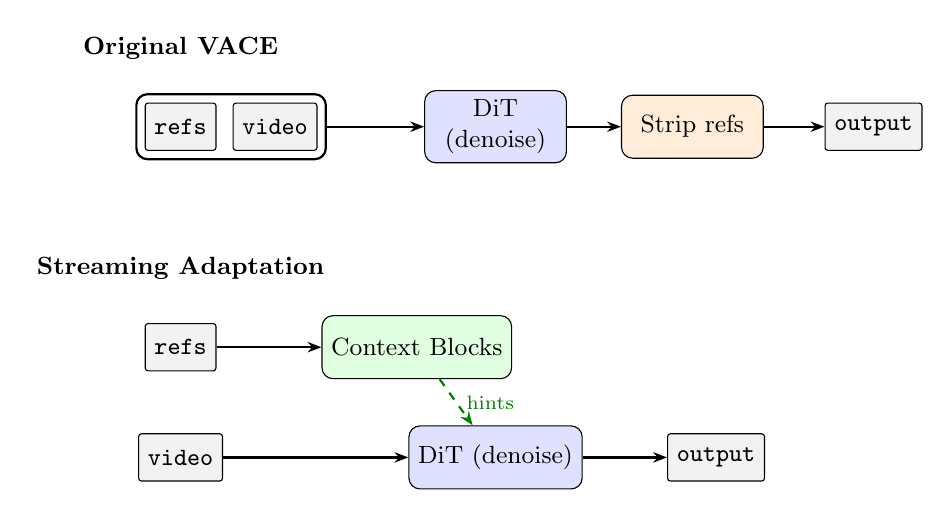
\begin{tikzpicture}[
    box/.style={draw, rounded corners, minimum height=0.8cm, minimum width=1.8cm, font=\small, align=center},
    data/.style={draw, rounded corners=1pt, minimum height=0.6cm, font=\small\ttfamily, fill=gray!10},
    arr/.style={-{Stealth[length=5pt]}, thick},
    darr/.style={-{Stealth[length=5pt]}, thick, dashed, color=green!50!black},
]
% === Original VACE (top row) ===
\node[font=\small\bfseries] at (0, 0) (orig-label) {Original VACE};

\node[data] at (0, -1) (refs1) {refs};
\node[data] at (1.2, -1) (vid1) {video};
\node[draw, thick, rounded corners, fit=(refs1)(vid1), inner sep=3pt] (concat) {};

\node[box, fill=blue!12] at (4, -1) (denoise1) {DiT\\(denoise)};
\node[box, fill=orange!15] at (6.5, -1) (strip) {Strip refs};
\node[data] at (8.8, -1) (out1) {output};

\draw[arr] (concat) -- (denoise1);
\draw[arr] (denoise1) -- (strip);
\draw[arr] (strip) -- (out1);

% === Streaming Adaptation (bottom rows) ===
\node[font=\small\bfseries] at (0, -2.8) (adapt-label) {Streaming Adaptation};

% Reference path (top of the two)
\node[data] at (0, -3.8) (refs2) {refs};
\node[box, fill=green!12] at (3, -3.8) (ctx) {Context Blocks};

% Video path (bottom of the two)
\node[data] at (0, -5.2) (vid2) {video};
\node[box, fill=blue!12] at (4, -5.2) (denoise2) {DiT (denoise)};
\node[data] at (6.8, -5.2) (out2) {output};

\draw[arr] (refs2) -- (ctx);
\draw[arr] (vid2) -- (denoise2);
\draw[darr] (ctx) -- node[right, font=\scriptsize, color=green!50!black] {hints} (denoise2);
\draw[arr] (denoise2) -- (out2);

\end{tikzpicture}
\caption{Original VACE concatenates references into the latent sequence, requiring post-hoc stripping. The streaming adaptation processes references through separate Context Blocks that inject hints into the DiT pathway, preserving fixed chunk sizes.}
\label{fig:arch}
\end{figure}

\section{Why Pretrained Weights Transfer}

The publicly released VACE weights use Context Adapter Tuning: the base DiT is frozen, and separate Context Blocks are trained to process conditioning inputs and inject hints. The Context Blocks are already trained to:

\begin{itemize}
    \item Encode reference information into a representation suitable for hint generation
    \item Generate hints that modulate the main DiT pathway
    \item Apply zero-initialized projections for controlled influence
\end{itemize}

\begin{table}[h]
\centering
\caption{Comparison of original VACE and the streaming adaptation.}
\label{tab:comparison}
\begin{tabular}{lll}
\toprule
\textbf{Component} & \textbf{Original VACE} & \textbf{Streaming Adaptation} \\
\midrule
Reference input & Concatenated into noisy latents & Separate conditioning tensor \\
Context Block inputs & Full sequence (refs + video) & References only \\
Hint injection target & Mixed ref+video sequence & Video-only sequence \\
Attention pattern & Bidirectional & Causal \\
\bottomrule
\end{tabular}
\end{table}

The Context Blocks themselves are unchanged---they process references and produce hints using the same weights. The adaptation changes \emph{where} references enter the pipeline and \emph{where} hints are injected.

The zero-initialized projections are critical to this transfer: at initialization they contribute nothing, and the trained weights encode learned scaling factors that remain valid in the adapted architecture.

\section{Streaming Compatibility and Capabilities}

Most VACE primitives transfer to streaming contexts with minimal adaptation. Masks, control signals (depth, pose, optical flow, scribble, grayscale, layout), dual-stream encoding, and hint injection all function with the same core mechanisms---requiring only cache management changes, not architectural ones. Reference image handling is the exception, addressed in Section~\ref{sec:adaptation}.

\begin{table}[h]
\centering
\caption{Streaming compatibility of VACE components.}
\label{tab:compat}
\begin{tabular}{lll}
\toprule
\textbf{Component} & \textbf{Compatibility} & \textbf{Notes} \\
\midrule
Masks & Full & Cache management for temporal autoencoders \\
Control signals (depth, pose) & Full & Per-chunk processing, same encoding \\
Dual-stream encoding & Full & Cache separation prevents contamination \\
Hint injection & Full & Residual addition unchanged \\
Reference images & Requires adaptation & Architectural change (Section~3.2) \\
\bottomrule
\end{tabular}
\end{table}

The adaptation supports structural control (V2V), masked generation including inpainting and outpainting (MV2V), temporal extension, experimental reference-to-video (R2V), and arbitrary compositions of these modes. Dynamic masks can be driven by real-time object detectors such as YOLO~\citep{jocher2026yolo26}, and inpainting composes with LoRA~\citep{hu2022lora} for regional style transfer. Mode is inferred from provided inputs with no explicit mode parameter. Figure~\ref{fig:pipeline} shows the per-chunk processing flow; Figures~\ref{fig:structural} and~\ref{fig:qualitative} show representative outputs.

\begin{figure}[h]
\centering
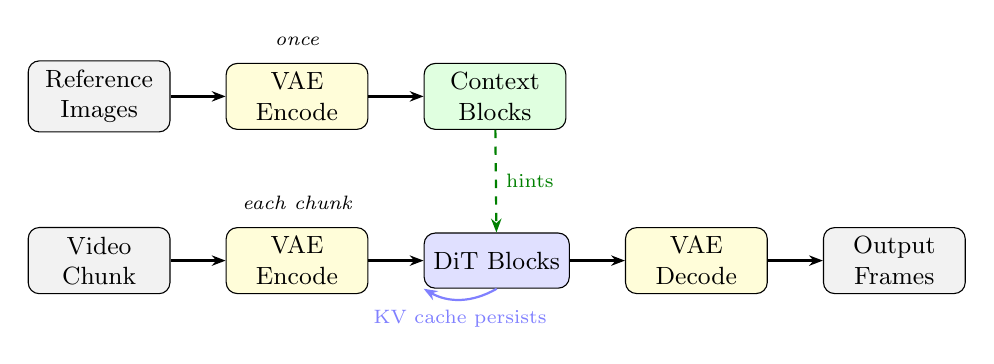
\begin{tikzpicture}[
    node distance=0.5cm and 0.7cm,
    box/.style={draw, rounded corners, minimum height=0.7cm, minimum width=1.8cm, font=\small, align=center},
    arr/.style={-{Stealth[length=5pt]}, thick},
    darr/.style={-{Stealth[length=5pt]}, thick, dashed, color=green!50!black},
]
% Top: reference path (once)
\node[box, fill=gray!10] (ref) {Reference\\Images};
\node[box, right=of ref, fill=yellow!15] (vae-ref) {VAE\\Encode};
\node[box, right=of vae-ref, fill=green!12] (ctx) {Context\\Blocks};

\draw[arr] (ref) -- (vae-ref);
\draw[arr] (vae-ref) -- (ctx);

% Label
\node[font=\scriptsize\itshape, above=0.1cm of vae-ref] {once};

% Bottom: video path (each chunk)
\node[box, below=1.2cm of ref, fill=gray!10] (chunk) {Video\\Chunk};
\node[box, right=of chunk, fill=yellow!15] (vae-vid) {VAE\\Encode};
\node[box, right=of vae-vid, fill=blue!12] (dit) {DiT Blocks};
\node[box, right=of dit, fill=yellow!15] (dec) {VAE\\Decode};
\node[box, right=of dec, fill=gray!10] (out) {Output\\Frames};

\draw[arr] (chunk) -- (vae-vid);
\draw[arr] (vae-vid) -- (dit);
\draw[arr] (dit) -- (dec);
\draw[arr] (dec) -- (out);

% Label
\node[font=\scriptsize\itshape, above=0.1cm of vae-vid] {each chunk};

% Hint injection
\draw[darr] (ctx) -- node[right, font=\scriptsize, color=green!50!black] {hints} (dit);

% KV cache
\draw[arr, color=blue!50, bend left=30] (dit.south) to node[below, font=\scriptsize, color=blue!50] {KV cache persists} (dit.south west);

\end{tikzpicture}
\caption{Per-chunk processing in the streaming VACE adaptation. Reference images are encoded once by Context Blocks; hints are injected into DiT blocks for each video chunk. The KV cache persists across chunks for autoregressive continuity.}
\label{fig:pipeline}
\end{figure}

\begin{figure}[H]
\centering
\setlength{\tabcolsep}{1pt}
\renewcommand{\arraystretch}{0.5}
\begin{tabular}{cccc}
& \small Input & \small Conditioning & \small Output \\[2pt]
\rotatebox{90}{\small ~~Depth} &
\includegraphics[width=0.17\textwidth]{figures/depth_comparison_left.jpg} &
\includegraphics[width=0.17\textwidth]{figures/depth_comparison_center.jpg} &
\includegraphics[width=0.17\textwidth]{figures/depth_comparison_right.jpg} \\[1pt]
\rotatebox{90}{\small ~~Scribble} &
\includegraphics[width=0.17\textwidth]{figures/scribble_comparison_low_strength_left.jpg} &
\includegraphics[width=0.17\textwidth]{figures/scribble_comparison_low_strength_center.jpg} &
\includegraphics[width=0.17\textwidth]{figures/scribble_comparison_low_strength_right.jpg} \\[1pt]
\rotatebox{90}{\small ~~Flow} &
\includegraphics[width=0.17\textwidth]{figures/optical_fish_comparison_left.jpg} &
\includegraphics[width=0.17\textwidth]{figures/optical_fish_comparison_center.jpg} &
\includegraphics[width=0.17\textwidth]{figures/optical_fish_comparison_right.jpg} \\[1pt]
\rotatebox{90}{\small ~~Color} &
\includegraphics[width=0.17\textwidth]{figures/gray_comparison_left.jpg} &
\includegraphics[width=0.17\textwidth]{figures/gray_comparison_center.jpg} &
\includegraphics[width=0.17\textwidth]{figures/gray_comparison_right.jpg} \\
\end{tabular}
\caption{Structural control modes. Each row: input frame, extracted conditioning signal, and generated output. Depth, scribble/edge, optical flow, and colorization (grayscale) controls shown.}
\label{fig:structural}
\end{figure}

\begin{figure}[H]
\centering
\setlength{\tabcolsep}{1pt}
\renewcommand{\arraystretch}{0.5}
\begin{tabular}{cccc}
& \small Input & \small Mask/Control & \small Output \\[2pt]
\rotatebox{90}{\small ~~Inpaint} &
\includegraphics[width=0.17\textwidth]{figures/inpainting_comparison_left.jpg} &
\includegraphics[width=0.17\textwidth]{figures/inpainting_comparison_center.jpg} &
\includegraphics[width=0.17\textwidth]{figures/inpainting_comparison_right.jpg} \\[1pt]
\rotatebox{90}{\small ~~LoRA} &
\includegraphics[width=0.17\textwidth]{figures/lora_comparison_left.jpg} &
\includegraphics[width=0.17\textwidth]{figures/lora_comparison_center.jpg} &
\includegraphics[width=0.17\textwidth]{figures/lora_comparison_right.jpg} \\[1pt]
\rotatebox{90}{\small ~~Layout} &
\includegraphics[width=0.17\textwidth]{figures/layout_comparison_left.jpg} &
\includegraphics[width=0.17\textwidth]{figures/layout_comparison_center.jpg} &
\includegraphics[width=0.17\textwidth]{figures/layout_comparison_right.jpg} \\[1pt]
& \small Input & & \small Output \\[2pt]
\rotatebox{90}{\small ~~I2V} &
\includegraphics[width=0.17\textwidth]{figures/i2v_comparison_left.jpg} &
&
\includegraphics[width=0.17\textwidth]{figures/i2v_comparison_right.jpg} \\[1pt]
\rotatebox{90}{\small ~~Outpaint} &
\includegraphics[width=0.17\textwidth]{figures/outpainting_comparison_left.jpg} &
&
\includegraphics[width=0.17\textwidth]{figures/outpainting_comparison_right.jpg} \\
\end{tabular}
\caption{Masked generation, layout control, and temporal extension. All outputs generated in real-time.}
\label{fig:qualitative}
\end{figure}

\section{Implementation}

The adaptation is implemented as a pipeline mixin compatible with multiple Wan-based autoregressive pipelines:

\begin{table}[h]
\centering
\caption{Validated base pipelines.}
\label{tab:pipelines}
\begin{tabular}{ll}
\toprule
\textbf{Base Pipeline} & \textbf{Reference} \\
\midrule
LongLive & \citep{yang2026longlive} \\
StreamDiffusion V2 & \citep{feng2025streamdiffusionv2} \\
MemFlow & \citep{ji2025memflow} \\
Krea Realtime Video & \citep{millon2025krea} \\
Reward Forcing & \citep{lu2025rewardforcing} \\
\bottomrule
\end{tabular}
\end{table}

Key design decisions include: separate VAE encoder caches for dual-stream encoding without temporal contamination; zero-initialized hint projections enabling safe composition with LoRA and quantization; implicit mode detection from provided inputs; crop-to-fill resizing to avoid padding artifacts; and cached hint computation where reference hints are computed once and reused across chunks.

\section{Performance}

Benchmarks were measured on a single NVIDIA RTX 5090 (32\,GB) with SageAttention~\citep{zhang2025sageattention} enabled. All models use bfloat16 precision at $368 \times 640$ resolution with TAE decoder. Each configuration was run for 15 measured chunks after 3 warmup chunks. These are inference-only measurements; end-to-end throughput with streaming overhead is slightly lower.

To validate cross-model compatibility, we benchmark on two Wan2.1 model scales: LongLive (1.3B, 4 denoising steps, 12 frames per chunk) and Krea Realtime Video (14B). The same VACE adaptation code is used for both without modification.

\begin{table}[h]
\centering
\caption{LongLive 1.3B ablation (12 frames per chunk, 4 denoising steps).}
\label{tab:perf-longlive}
\begin{tabular}{lcccc}
\toprule
\textbf{Configuration} & \textbf{Avg Latency} & \textbf{Avg FPS} & \textbf{Peak FPS} & \textbf{Peak VRAM} \\
\midrule
Baseline (no VACE) & 539\,ms & 22.3 & 22.8 & 13.2\,GB \\
+ Depth Control & 698\,ms & 17.2 & 17.4 & 14.6\,GB \\
+ Inpainting & 698\,ms & 17.2 & 17.3 & 14.6\,GB \\
+ Extension (I2V) & 534\,ms & 22.5 & 22.7 & 14.6\,GB \\
\bottomrule
\end{tabular}
\end{table}

\begin{table}[h]
\centering
\caption{Krea Realtime Video 14B ablation (TODO: frames per chunk, TODO denoising steps, TODO resolution).}
\label{tab:perf-krea}
\begin{tabular}{lcccc}
\toprule
\textbf{Configuration} & \textbf{Avg Latency} & \textbf{Avg FPS} & \textbf{Peak FPS} & \textbf{Peak VRAM} \\
\midrule
Baseline (no VACE) & TODO & TODO & TODO & TODO \\
+ Depth Control & TODO & TODO & TODO & TODO \\
+ Inpainting & TODO & TODO & TODO & TODO \\
+ Extension (I2V) & TODO & TODO & TODO & TODO \\
\bottomrule
\end{tabular}
\end{table}

VACE adds approximately 1.4\,GB of VRAM overhead for the 1.3B model (the VACE Context Block weights). Per-chunk latency overhead varies by mode. With LongLive (4 denoising steps), VACE context encoding adds ${\sim}$30\% latency for depth and inpainting. Extension mode caches reference hints after the first chunk, resulting in negligible overhead (${\sim}$1\%) for subsequent chunks.

% TODO: Add Krea 14B performance discussion once benchmarks are available.

\section{Related Work}

The primary alternative for real-time controlled video generation is MotionStream~\citep{shin2025motionstream}, a fully distilled model with built-in trajectory control. MotionStream achieves higher quality for its specific control modality but requires full model retraining for each control type.

This adaptation trades some per-task quality for versatility: a single set of pretrained weights enables depth control, scribble guidance, inpainting, layout control, and arbitrary combinations without retraining. The approach extends to new control types as they are developed for batch VACE.

\section{Limitations}

\begin{itemize}
    \item \textbf{Temporal coherence} can degrade over extended generations ($100$+ frames) without re-anchoring---a general consequence of autoregressive generation.
    \item \textbf{Control signal variance:} Some signals (depth, scribble, layout) work reliably; others require more tuning.
    \item \textbf{Reference-to-Video} is the most problematic capability. Detail preservation and reference fidelity are severely degraded compared to batch VACE due to causal attention and per-chunk processing. Further architectural work is needed.
    \item \textbf{First+last frame extension} has reduced utility compared to batch VACE due to small chunk sizes in streaming contexts.
    \item \textbf{No perceptual quality metrics} (FVD, FID) comparing to batch VACE are provided. Throughput and overhead are measured but visual quality comparison is left to future work.
\end{itemize}

\section{Conclusion}

By moving reference frames from the diffusion latent space into a parallel conditioning pathway, this adaptation preserves the fixed chunk sizes and KV caching that autoregressive models require while reusing existing VACE weights directly. Structural control, masked generation, and temporal extension function at real-time rates (17--22 FPS) on consumer hardware. The approach has been validated across Wan2.1 1.3B and 14B model scales without per-model modifications.

\section*{Acknowledgements}

The author thanks Yondon Fu, Rafal Leszko, and Marco Tundo for their support and feedback throughout this work.

\bibliographystyle{plainnat}
\bibliography{references}

\end{document}
